\documentclass[11pt]{article}

\usepackage[margin=1in]{geometry}
\usepackage{lmodern}
\usepackage{graphicx}
\usepackage{booktabs}
\usepackage{amsmath,amssymb}
\usepackage{natbib}
\usepackage[hidelinks]{hyperref}
\usepackage{xcolor}
\usepackage{setspace}
\usepackage{caption}
\captionsetup{font=small,labelfont=bf}

\setstretch{1.08}
\bibliographystyle{plainnat}

\title{Evidence Helps on Average, but Sometimes Hurts:\\
Diagnosing Evidence-Induced Regressions in LLM Fact Verification}

\author{
Chimdumebi Mitchell Nebolisa\\
\textit{Affiliation TODO}\\
\and
Jessica Udry\\
\textit{Affiliation TODO}
}

\date{Manuscript draft for internal review\\[0.4em]
\small Frozen artifact: \texttt{evidex-artifact-v1} (\texttt{29102c3})\\
Venue-neutral first draft. Not a submission.}

\begin{document}
\maketitle

\begin{abstract}
Supplying designated gold evidence is widely assumed to make language-model fact verification more reliable.
We test that assumption in a paired experiment on 10{,}000 balanced FEVER Supported/Refuted claims, evaluating GPT-5.4 and GPT-5.4-mini without evidence and with FEVER-designated gold evidence (40{,}000 predictions).
Evidence raises aggregate accuracy from 88.69\% to 96.04\% ($+7.35$~pp) for GPT-5.4 and from 84.67\% to 95.54\% ($+10.87$~pp) for GPT-5.4-mini.
Those gains conceal a structured minority of evidence-induced regressions: 226 unique claims that were correct without evidence become wrong after the same gold evidence is supplied (40 shared by both models; 186 specific to one model).
Blinded five-judge progressive-disclosure adjudication on the diagnostic cohort decomposes those regressions into a mixture of evidence-utilization failure, residual warrant ambiguity, and representation-sensitive behavior.
A Cursor/Grok panel assigns 50.0\% / 11.9\% / 38.1\% of the 226 regressions to those categories.
An independent Claude five-judge A$\rightarrow$B$\rightarrow$C replication on the same 226 items (3{,}390 judgments) recovers the same qualitative ordering but not the same prevalences (65.9\% / 5.3\% / 28.8\%; exact taxonomy agreement 74.3\%, $\kappa=0.537$).
External evidence can therefore improve overall reliability while creating localized failures, and automated failure-mode prevalence itself depends partly on the adjudicating model family.

\end{abstract}

\noindent\textit{Keywords:} fact verification, FEVER, large language models, evidence utilization, silver adjudication, LLM-as-judge

\section{Introduction}
\label{sec:intro}

Evidence grounding is a standard recipe for making language-model fact verification more trustworthy.
If a model is shown the same designated evidence that a benchmark treats as sufficient, aggregate accuracy should rise, and remaining errors should look like residual retrieval or coverage problems rather than failures to use gold evidence.
That picture is incomplete.
Aggregate improvements can hide a second phenomenon: claims the model already answered correctly without evidence, then answered incorrectly after the designated evidence was added.

This paper studies that phenomenon on FEVER \citep{thorne-etal-2018-fever}.
We evaluate GPT-5.4 and GPT-5.4-mini on a balanced 10{,}000-claim Supported/Refuted sample under two paired conditions: claim only, and claim plus FEVER-designated gold evidence.
Evidence helps in aggregate (Table~\ref{tab:accuracy}).
It also induces 226 unique correct-to-wrong regressions.
Those regressions are rare relative to the 10{,}000-claim sample, but they are not unstructured noise.
They concentrate on claim--evidence pairs that local NLI models treat as weakly warranted, and they are only partly shared across the two GPT models.

Counting regressions is not enough.
The same behavioral pattern can arise from at least three diagnostic situations: the model fails to use evidence that a later adjudicator finds decisive; the evidence representation (sentence text versus titles versus structured provenance) changes the warrant; or the claim--evidence pair remains underdetermined after full designated evidence is shown.
We therefore run blinded progressive-disclosure silver adjudication.
Five isolated judges see sentence evidence (Stage~A), then page titles (Stage~B), then reconstructed structured FEVER evidence (Stage~C).
A rule-based taxonomy maps consensus transitions onto three broad diagnostic categories: evidence-utilization failure, representation-sensitive behavior, and residual ambiguity.
The primary panel uses one locked Cursor/Grok model.
Supporting checks include a GLM-5.3 Stage~A replication and a Claude Stage~C test on 231 Grok leftovers.
The decisive robustness experiment is a complete Claude A$\rightarrow$B$\rightarrow$C panel on all 226 regressions.

The resulting claim is two-part.
First, designated gold evidence improves overall accuracy while creating a measurable set of localized regressions whose diagnostic picture is mixed rather than single-cause.
Second, that mixed picture is qualitatively stable across judge families, but exact category prevalences are not.
Automated diagnostic decompositions therefore carry measurement uncertainty of their own.

\paragraph{Contributions.}
We (i)~quantify paired evidence gains and evidence-induced regressions on a verified 10{,}000-claim FEVER experiment;
(ii)~characterize regressions with confirmatory statistics, two local NLI diagnostics, and a 1{,}061-claim diagnostic cohort;
(iii)~decompose the 226 unique regressions with blinded progressive-disclosure silver adjudication; and
(iv)~show, with a 3{,}390-judgment Claude replication, which parts of that decomposition survive a change of adjudicating family.

We ask four research questions, restated in Section~\ref{sec:rqs}.
RQ1 asks whether designated gold evidence improves aggregate accuracy.
RQ2 asks how frequent and cross-model-consistent the regressions are.
RQ3 asks which diagnostic failure modes appear under progressive disclosure.
RQ4 asks which of those conclusions survive a change in judge family.

\section{Related Work}
\label{sec:related}

\subsection{Evidence-based fact verification}
Automated fact verification is commonly decomposed into claim detection, evidence retrieval, and verdict prediction \citep{guo-etal-2022-survey}.
FEVER \citep{thorne-etal-2018-fever} made the last two stages measurable at scale by pairing Wikipedia-derived claims with annotator-selected evidence sentences and ternary labels (Supported, Refuted, NotEnoughInfo).
The first shared task already showed that retrieval and verification are both hard even when the evidence corpus is Wikipedia \citep{thorne-etal-2018-fact}.
Later datasets extend the setting to scientific abstracts \citep{wadden-etal-2020-fact}, contrastive evidence revisions \citep{schuster-etal-2021-get}, many-hop Wikipedia evidence \citep{jiang-etal-2020-hover}, and mixed sentence/table evidence \citep{aly-etal-2021-feverous}.
Claim-only artifacts are also documented: models can exploit label cues that survive without evidence \citep{schuster-etal-2019-towards}.
Our experiment holds retrieval fixed: we supply FEVER-designated gold evidence and ask how an LLM uses it.
That isolates utilization and representation from open retrieval, at the cost of studying a 2017-era, Wikipedia-centric, binary Supported/Refuted slice of the original task.

\subsection{LLM reasoning with external evidence}
LLMs do not treat supplied context as an oracle.
Knowledge-conflict studies show that parametric memory can override or ignore contradictory context \citep{longpre-etal-2021-entity}.
Even when the relevant span is present, models are sensitive to where and how it is written \citep{liu-etal-2024-lost} and can be pulled off-task by irrelevant material \citep{shi2023distracted}.
Wan et al.\ \citep{wan-etal-2024-evidence} show that models overweight surface relevance relative to credibility cues that humans treat as important.
Mamta and Cocarascu \citep{mamta-cocarascu-2025-facteval} find that LLM fact verification on FEVER is brittle under small input perturbations.
These results motivate a paired no-evidence versus gold-evidence design: if designated evidence still produces regressions, the failure is not missing retrieval.

\subsection{Evidence sufficiency and ambiguity}
Presence of evidence is not sufficiency.
Atanasova et al.\ \citep{atanasova-etal-2022-fact} show that fact-checking models often fail to detect when remaining evidence is insufficient.
Glockner et al.\ \citep{glockner-etal-2024-ambifc} document claim--evidence pairs that admit conflicting but valid interpretations and argue against forcing a single hard label.
Our residual-ambiguity category is a silver-adjudicator analogue of that problem: after full designated evidence, a panel still withholds Supported/Refuted.
We do not treat that disagreement as proof that a FEVER label is wrong.

\subsection{LLM-as-judge and evaluator sensitivity}
Using LLMs as judges scales evaluation but imports judge-specific biases, including position, verbosity, and self-preference effects \citep{zheng2023judging,liu-etal-2023-g,chen-etal-2024-humans}.
Position bias itself varies by judge and task rather than appearing as a uniform artifact \citep{shi-etal-2025-judging}.
Huang et al.\ \citep{huang-etal-2025-empirical} show that judge models are not interchangeable substitutes for one another.
We therefore treat judge-family disagreement as a result.
Cursor/Grok and Claude are two silver instruments applied to the same blinded packets.
Agreement supports robustness of the qualitative taxonomy; disagreement bounds how precisely any one family can estimate category prevalence.
Neither panel is human ground truth.

\section{Study Design}
\label{sec:design}

\subsection{Research questions}
\label{sec:rqs}
\begin{description}
\item[RQ1] How does providing FEVER-designated gold evidence affect aggregate LLM fact-verification accuracy?
\item[RQ2] When evidence changes a previously correct prediction into an incorrect one, how frequent and consistent are those regressions across models?
\item[RQ3] What observable diagnostic failure modes characterize evidence-induced regressions under progressive disclosure?
\item[RQ4] Do those diagnostic conclusions survive a change in adjudicating model family?
\end{description}

\subsection{FEVER dataset and sampling}
We sample from the FEVER development set \citep{thorne-etal-2018-fever}.
The manuscript experiment is a balanced 10{,}000-claim extract: 5{,}000 Supported and 5{,}000 Refuted, seed 42, \texttt{NOT ENOUGH INFO} excluded.
Gold evidence is resolved from official FEVER Wikipedia shards into the text shown to the models.
Sampling and validation artifacts are committed with the frozen repository; third-party FEVER and Wikipedia text are not relicensed by the project MIT license.

\subsection{Models and paired evidence conditions}
Each claim is evaluated four times: GPT-5.4 and GPT-5.4-mini, each under \texttt{claim\_only} and \texttt{claim\_plus\_evidence}.
That yields 40{,}000 predictions.
The evidence condition uses the designated FEVER evidence, not an open-web retrieval step.
Original GPT runs stored labels only, so later analysis cannot recover confidence or token-level attributions.

\subsection{Transition definitions}
For each model, a claim has one of four paired transitions:
\emph{robust} (correct without and with evidence),
\emph{rescue} (wrong without, correct with),
\emph{resistant} (wrong in both),
or \emph{regression} (correct without, wrong with).
A unique-claim regression is a claim that regresses for at least one of the two GPT models.
Unique-claim counts are never treated as model-observations: 115 GPT-5.4 regressions and 151 mini regressions are 226 unique claims, not 266.

\subsection{Analysis v2}
Analysis v2 treats the 40{,}000-row experiment file as immutable source data.
It rebuilds the paired dataset, runs McNemar tests and bootstrap confidence intervals, extracts linguistic and evidence-structure features, embeds claim--evidence pairs, and applies two local NLI models (nli-deberta-v3-small and distilbert-base-uncased-mnli) as diagnostics, not as ground truth.
Leakage audits and an independent 69-check headline verifier are part of the frozen record.
Confirmatory tests were pre-specified; NLI and feature analyses are exploratory.

\subsection{Diagnostic cohort}
The adjudication cohort contains 1{,}061 unique claims: all 226 unique regressions, 335 resistant, 250 rescue, and 250 robust.
One item (\texttt{SA-000352}) is provider-filtered, so judged $N=1{,}060$.
The Claude full panel judges only the 226 regressions.
The Claude residual panel judges only the 231 Cursor/Grok Stage~C leftovers.
Those three samples answer different questions and are not interchangeable.

\subsection{Progressive-disclosure adjudication}
\label{sec:protocol}
Five isolated judges see nested evidence representations:
Stage~A, gold evidence sentences only;
Stage~B, Stage~A plus page titles;
Stage~C, reconstructed structured FEVER evidence (chosen set, alternatives, archive flags).
Judges do not browse, retrieve new pages, or see FEVER labels, GPT predictions, cohort tags, NLI scores, or other judges.
Stages are frozen before the next packets are built.
Consensus and the three-way taxonomy are computed by code.
We call the categories \emph{diagnostic failure modes}: they describe where a blinded panel's warrant changes, not a causal mechanism inside GPT.

The primary panel locks \texttt{cursor-grok-4.6-high-fast} for all judges and a same-family resolver on non-high-consensus items.
Taxonomy comparison with Claude uses consensus labels, which are computed identically across panels.

\subsection{Cross-family replication}
\label{sec:cross-family-design}
GLM-5.3 contributes a completed Stage~A panel compared to frozen Cursor Stage~A ($n=1{,}060$).
Partial GLM Stages~B and~C exist only as provenance and are excluded from A$\rightarrow$B$\rightarrow$C mathematics.

The Claude residual experiment is a Stage~C robustness test on the 231 Cursor/Grok Ambiguous/Unresolved leftovers (\texttt{claude-opus-5-thinking-high}, five judges, 1{,}155 judgments, no resolver).
It is selection-conditioned on Grok leftovers.

The main Claude experiment independently reruns A$\rightarrow$B$\rightarrow$C on all 226 unique regressions (226$\times$5$\times$3 $= 3{,}390$ judgments), with fresh opaque IDs and no splicing of residual-panel judgments.
During execution, the first Stage~A batch-01 wave used judge-facing paths that named the panel directory and therefore the cohort-selection criterion.
Those 385 judgments were quarantined unread, paths were replaced with a neutral \texttt{blind\_io} namespace, and the batch was rerun under the same locked model, rubric, and evidence packets.
A later usage-limit interruption paused Stage~B; work resumed on the same Claude slug, and already-valid judgments were retained.
Overlapping recovery produced three duplicate Stage~B judge-batches; a content-independent first-ingested-wins rule kept one copy.
Details are in Appendix~\ref{app:deviations}.

\subsection{Statistical analysis and verification}
Paired accuracy uses McNemar tests.
Regression and rescue rates use bootstrap confidence intervals.
Cross-family taxonomy agreement is reported as exact match, broad-category match, and Cohen's $\kappa$.
Stage-wise ambiguity differences use McNemar tests on the paired 226-item sample.
The frozen artifact verifies Analysis~v2 (69/69), Cursor/Grok (33/33), read-only GLM Stage~A, Claude residual (38/38), and Claude full (21/21).
Cohen's $\kappa=0.537$ is taken from the canonical synthesis, not from the Claude \texttt{HEADLINES.json} registry.


\begin{table}[t]
\centering
\caption{Paired behavioral results on 10{,}000 balanced FEVER Supported/Refuted claims (40{,}000 predictions). Accuracies and transition counts are from the verified Analysis~v2 tables. Unique-claim regression counts treat a claim as one unit even if both models regress.}
\label{tab:accuracy}
\begin{tabular}{lrrrrr}
\toprule
Model & Claim-only & +Gold ev. & $\Delta$ (pp) & Regressions & Rescues \\
\midrule
GPT-5.4 & 88.69\% & 96.04\% & $+7.35$ & 115 (1.15\%) & 850 (8.5\%) \\
GPT-5.4-mini & 84.67\% & 95.54\% & $+10.87$ & 151 (1.51\%) & 1{,}238 (12.4\%) \\
\midrule
\multicolumn{6}{l}{Unique claims that regress for at least one model: 226 (40 both; 186 exactly one).} \\
\bottomrule
\end{tabular}
\end{table}

\begin{table}[t]
\centering
\caption{Cursor/Grok diagnostic failure-mode assignment among the 226 unique regressions. Labels are rule-based summaries of blinded progressive-disclosure consensus, not human ground truth and not GPT-internal causes.}
\label{tab:mechanism-grok}
\begin{tabular}{lrr}
\toprule
Diagnostic category & $n$ & Share \\
\midrule
Evidence-utilization failure & 113 & 50.0\% \\
Representation-sensitive & 27 & 11.9\% \\
Residual ambiguity & 86 & 38.1\% \\
\bottomrule
\end{tabular}
\end{table}

\begin{table}[t]
\centering
\caption{Full-panel cross-family comparison on the same 226 regressions. Exact and broad taxonomy agreement are both 74.3\% (168/226); Cohen's $\kappa=0.537$ (moderate). These are silver-adjudicator agreements, not human prevalences.}
\label{tab:cross-family}
\begin{tabular}{lrrrr}
\toprule
Category & Grok $n$ & Grok \% & Claude $n$ & Claude \% \\
\midrule
Evidence-utilization failure & 113 & 50.0 & 149 & 65.9 \\
Representation-sensitive & 27 & 11.9 & 12 & 5.3 \\
Residual ambiguity & 86 & 38.1 & 65 & 28.8 \\
\bottomrule
\end{tabular}
\end{table}

\begin{table}[t]
\centering
\caption{Residual-ambiguity rates among shared versus model-specific regressions. Both families find shared regressions more persistently non-decisive. Absolute levels differ by family.}
\label{tab:shared}
\begin{tabular}{lrrr}
\toprule
Subgroup & $n$ & Grok residual amb. & Claude residual amb. \\
\midrule
Shared by both GPT models & 40 & 60.0\% & 47.5\% \\
Exactly one GPT model & 186 & 33.3\% & 24.7\% \\
\bottomrule
\end{tabular}
\end{table}


\section{Results}
\label{sec:results}

\subsection{Gold evidence improves aggregate accuracy}
\label{sec:rq1}
Table~\ref{tab:accuracy} answers RQ1.
On the same 10{,}000 claims, designated gold evidence raises GPT-5.4 accuracy from 88.69\% to 96.04\% ($+7.35$~pp) and GPT-5.4-mini from 84.67\% to 95.54\% ($+10.87$~pp).
Paired McNemar tests are large (GPT-5.4 $\chi^2=558.3$, $p\approx 2\times 10^{-123}$; mini $\chi^2=849.1$, $p\approx 10^{-186}$).
Figure~\ref{fig:transitions} shows the four-way transition structure behind those averages.
Evidence also increases cross-model prediction agreement, from 89.3\% ($\kappa=0.786$) without evidence to 97.2\% ($\kappa=0.944$) with evidence.

\begin{figure}[t]
\centering
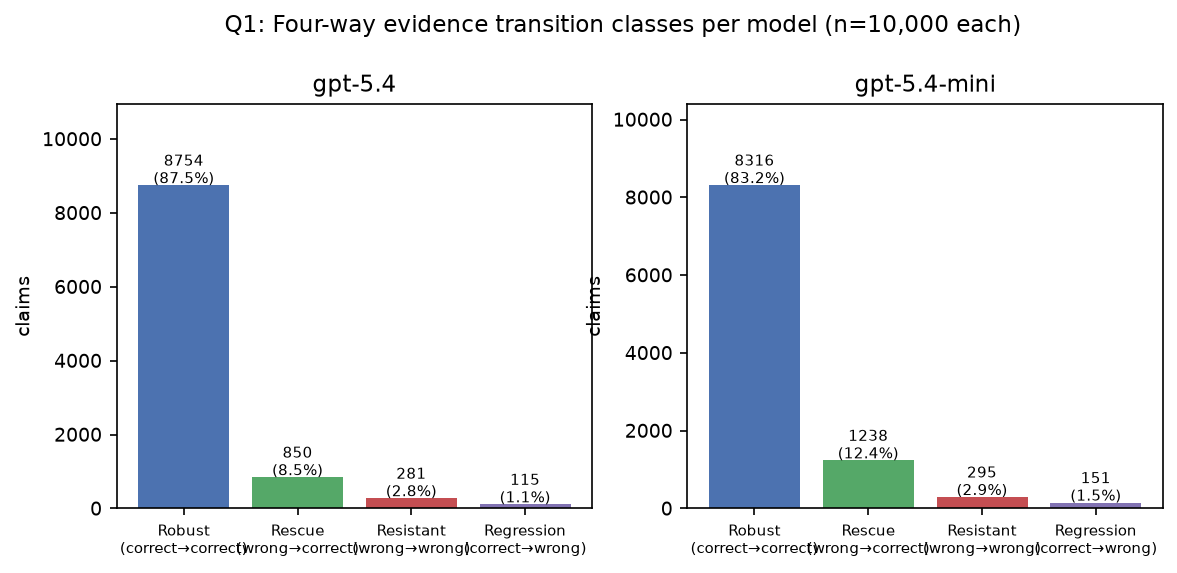
\includegraphics[width=0.92\linewidth]{../analysis_v2/figures/fig1_transition_matrices.png}
\caption{Paired transition matrices for GPT-5.4 and GPT-5.4-mini. Off-diagonal cells are rescues (wrong$\rightarrow$correct) and regressions (correct$\rightarrow$wrong).}
\label{fig:transitions}
\end{figure}

\subsection{Evidence can induce correct-to-wrong regressions}
\label{sec:rq2}
The same paired design produces 115 GPT-5.4 regressions (1.15\%, bootstrap 95\% CI $[0.95,1.36]$) and 151 mini regressions (1.51\%, CI $[1.28,1.75]$).
Rescues are more common: 850 (8.5\%) and 1{,}238 (12.4\%).
Among claim-only errors, evidence corrects 75.2\% (GPT-5.4) and 80.8\% (mini).

Unique-claim counts, not model-observations, are the regression cohort for later adjudication: 226 claims regress for at least one model, 40 for both, and 186 for exactly one (75 GPT-5.4-only, 111 mini-only).
A paired McNemar test on discordant claims finds a modest model difference in regression incidence (115 vs.\ 151, $\chi^2=6.59$, $p=0.010$).
87.3\% of claims share the same transition class across models.
RQ2's answer is therefore: regressions are real, rare relative to 10{,}000 claims, only partly shared, and large enough to study as a structured minority.

\subsection{Characteristics of evidence-induced regressions}
\label{sec:rq3-nli}
Regressions are not a random slice of the sample.
A local NLI diagnostic (nli-deberta-v3-small) disagrees with the FEVER label on 74.8\% of GPT-5.4 regressions and 76.8\% of mini regressions, against 22.6\% of GPT-5.4 robust successes (Figure~\ref{fig:nli}).
Resistant failures look similar (75.8\%).
A second, architecturally different NLI model reproduces the same ordering.
The 2{,}462 claims flagged as weakly warranted also have lower claim-only GPT-5.4 accuracy (81.0\% vs.\ 88.69\%), so the NLI signal marks hard items rather than a quirk of one evidence-condition model.

\begin{figure}[t]
\centering
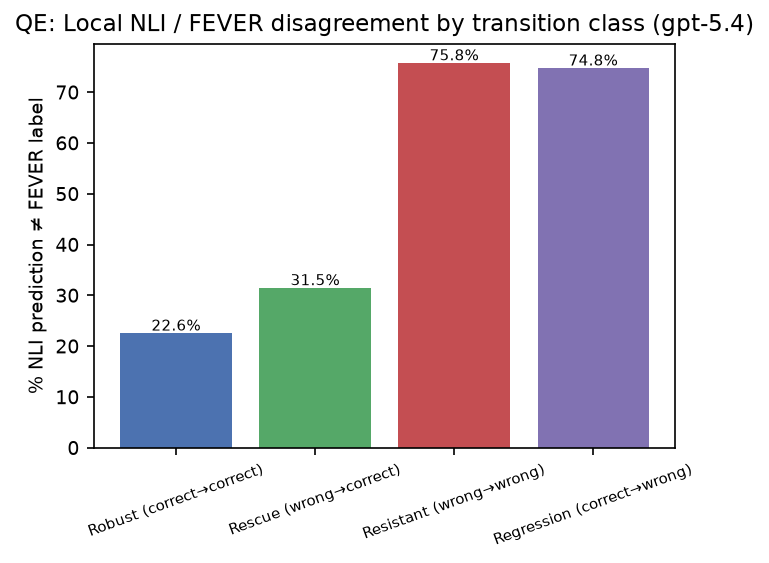
\includegraphics[width=0.88\linewidth]{../analysis_v2/figures/fig6_nli_disagreement.png}
\caption{Local NLI disagreement with the FEVER label by GPT-5.4 transition class. The NLI models are diagnostics, not a relabeling of FEVER.}
\label{fig:nli}
\end{figure}

Label asymmetry is model-dependent.
GPT-5.4 regressions concentrate on Supported claims (88 vs.\ 27 Refuted, $p=1.8\times 10^{-8}$); mini shows no such split (74 vs.\ 77, $p=0.87$).
Surface features (length, overlap, evidence-set size) only weakly separate regressions.
Predictive models that include NLI features do better than surface-only models, but rare-class PR-AUC remains low.
We treat this block as characterization, not as the failure-mode decomposition.

\subsection{Progressive disclosure reveals a mixed failure picture}
\label{sec:rq3-grok}
The Cursor/Grok panel judges the 1{,}061-claim cohort (judged $N=1{,}060$).
Among the 226 regressions, the rule-based taxonomy yields a mixed assignment (Table~\ref{tab:mechanism-grok}): 50.0\% evidence-utilization failure, 11.9\% representation-sensitive, 38.1\% residual ambiguity.
Utilization failure means the panel reaches a high-consensus decisive Stage~C verdict on evidence the GPT model used incorrectly.
Residual ambiguity means the panel remains Ambiguous or Unresolved after structured evidence.
Representation-sensitive items become decisive only after titles or structure are added.

Progressive disclosure itself resolves only a minority of regression ambiguity (7.1\% by titles, 5.3\% only by structure).
No decisive consensus is reversed by later disclosure.
Shared GPT regressions remain more often non-decisive than model-specific ones (Table~\ref{tab:shared}).
This is the Grok answer to RQ3: a mixture, with utilization largest and representation smallest, not a single-cause story.

\subsection{Supporting cross-family checks}
\label{sec:supporting}
GLM-5.3 Stage~A, compared with frozen Cursor Stage~A on 1{,}060 items, yields modal verdict agreement 0.862 and consensus agreement 0.831.
GLM is less ambiguity-conservative (ambiguous/unresolved rate 0.223 vs.\ Cursor 0.291).
This is Stage~A robustness only.

The Claude residual Stage~C test on 231 Grok leftovers finds persistent ambiguity on 134/231 (58.0\%, CI $51.5$--$64.1$) and Claude-resolved Grok leftovers on 97/231 (42.0\%).
The leftover set is therefore mixed: most of it still looks underdetermined to a second family, and a large high-consensus slice does not.
This experiment cannot re-open the 113 Grok utilization failures or the 27 representation-sensitive items, because those items were not in the residual sample.

\subsection{Full Claude replication}
\label{sec:rq4}
The complete Claude A$\rightarrow$B$\rightarrow$C panel judges all 226 regressions from scratch (3{,}390 judgments).
Table~\ref{tab:cross-family} and Figure~\ref{fig:by-family} are the study-level comparison.
Claude assigns 65.9\% utilization failure (149), 5.3\% representation-sensitive (12), and 28.8\% residual ambiguity (65).
The rank order matches Grok.
The magnitudes do not: Claude's utilization share is 15.9~pp higher, and the reported 95\% intervals (Claude $59.5$--$71.8$; Grok $43.5$--$56.5$) do not overlap.

\begin{figure}[t]
\centering
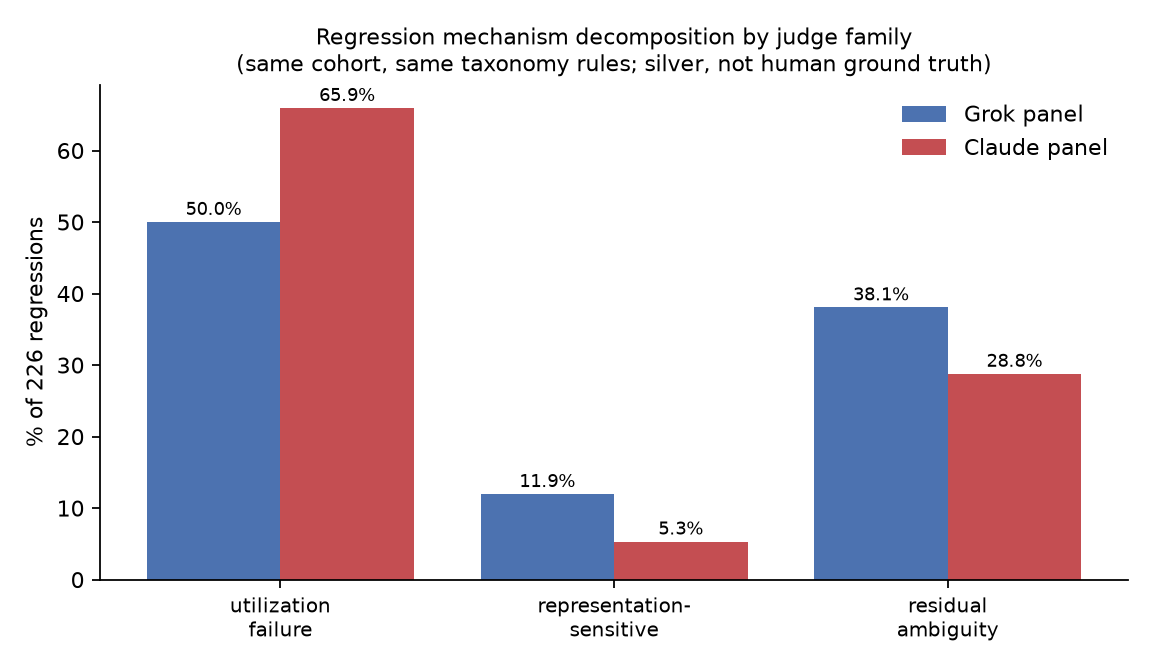
\includegraphics[width=0.92\linewidth]{../silver_adjudication_v1/claude_full_regression_panel/figures/fig1_mechanism_by_family.png}
\caption{Diagnostic category shares for the same 226 regressions under Cursor/Grok and Claude. Ordering matches; prevalences do not.}
\label{fig:by-family}
\end{figure}

Exact taxonomy agreement is 74.3\% (168/226); broad-category agreement is also 74.3\%, because neither panel assigns \texttt{silver\_title\_context\_sensitive}.
Cohen's $\kappa=0.537$ (moderate).
Disagreement is directional.
Claude reclassifies 20 of Grok's 27 representation-sensitive items and 22 of Grok's 86 residual items as utilization failures, and moves only six items the other way.
Claude retains 4 of Grok's 27 representation-sensitive cases.

\begin{figure}[t]
\centering
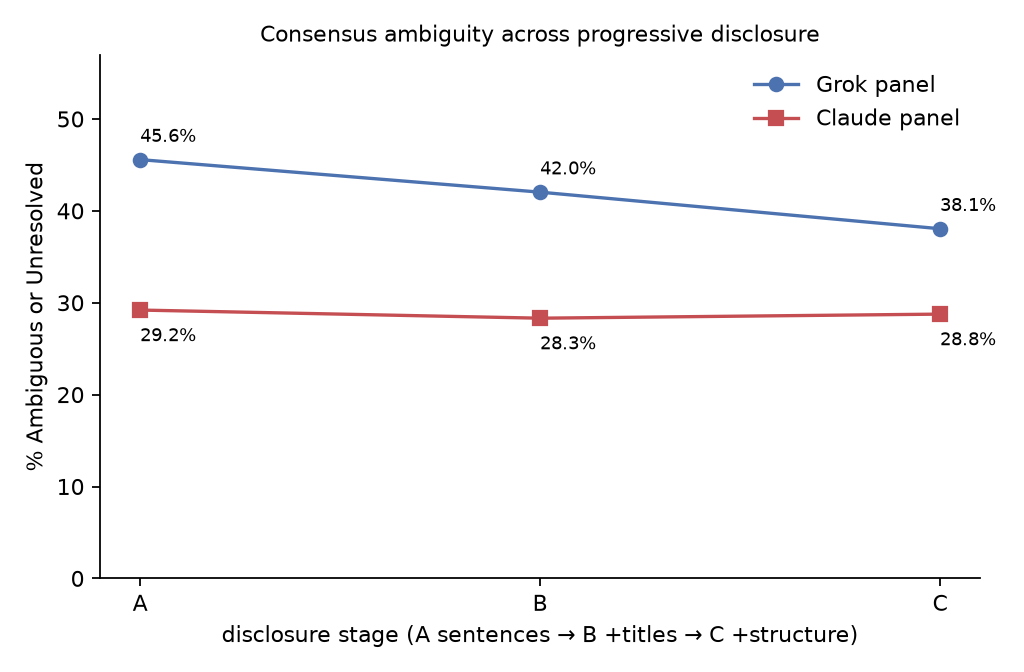
\includegraphics[width=0.88\linewidth]{../silver_adjudication_v1/claude_full_regression_panel/figures/fig2_stage_ambiguity.png}
\caption{Stage-wise non-decisive rates on the 226 regressions. Claude is more decisive at every stage; the gap narrows from Stage~A to Stage~C. Title and structure disclosure resolve only a small share in both families.}
\label{fig:stage-amb}
\end{figure}

Figure~\ref{fig:stage-amb} shows the stage-level mechanism behind that shift.
Claude's ambiguity rate is lower at every stage (29.2\% / 28.3\% / 28.8\% vs.\ Grok 45.6\% / 42.0\% / 38.1\%; McNemar $p=7.8\times 10^{-10}$, $3.4\times 10^{-7}$, $7.5\times 10^{-4}$).
Title and structure resolution rates do not differ significantly across families.
Neither family reverses a decisive consensus after added disclosure.
Shared regressions remain stickier than model-specific ones under Claude as well (Table~\ref{tab:shared}).

\subsection{What replicates and what does not}
\label{sec:what-replicates}
Robust across both complete panels: all three diagnostic categories occur; utilization failure is largest; residual ambiguity remains substantial; representation-sensitive cases are smallest; additional disclosure resolves only a minority; decisive consensus is never reversed; shared regressions are more ambiguity-prone.

Quantitatively offset but directionally consistent: the utilization-versus-residual split, and stage-wise ambiguity (same trend, 9--16~pp lower under Claude).

Judge-family-sensitive: absolute ambiguity at every stage; the representation-sensitive item set (4-item overlap); and per-claim assignment ($\kappa=0.537$).
RQ4's answer is therefore qualitative yes, quantitative no.
The design cannot decide whether Claude is better calibrated or more overconfident on thin warrants, because both panels are models scoring the same packets.

\section{Discussion}
\label{sec:discussion}

\subsection{Evidence helps globally but can hurt locally}
The practical headline is not that gold evidence fails.
It succeeds on average, and it rescues far more claim-only errors than it creates.
The scientific headline is that those averages are the wrong unit for reliability engineering.
A 1.15--1.51\% regression rate is small in a 10{,}000-claim table and large if each regression is a previously correct decision that evidence reversed.
Evaluation reports that publish only condition-wise accuracy will miss that reversal.

\subsection{Evidence availability versus evidence utilization}
Half or more of the 226 regressions are labeled utilization failures by at least one complete panel.
On those items a blinded adjudicator finds the designated evidence decisive after Stage~C, while the original GPT model flipped away from the correct label when that evidence was added.
This is closer to a use failure than to a missing-evidence failure.
It sits next to work showing that models can ignore, mishandle, or be distracted by context they were given \citep{longpre-etal-2021-entity,shi2023distracted,wan-etal-2024-evidence}.
We still cannot say \emph{why} GPT flipped: the original runs stored labels only.

\subsection{Ambiguity and representation sensitivity}
Residual ambiguity is the second category in both families.
That is expected given prior evidence that sufficiency and ambiguity are first-class problems in fact verification \citep{atanasova-etal-2022-fact,glockner-etal-2024-ambifc}.
We do not interpret residual silver ambiguity as a FEVER annotation error.
Representation-sensitive cases are the smallest bucket in both families, and the item-level set is unstable (4 shared of 27 Grok cases).
Titles and structure help some items and never reverse a decisive consensus.
That supports a cautious claim: representation matters, but it is not the main quantitative story, and it is the least portable category across judge families.

\subsection{Judge-family dependence as measurement uncertainty}
The Claude-versus-Grok gap is the second contribution, not a defect to be explained away.
LLM-as-judge work already shows that evaluators have family-specific biases and are not drop-in substitutes \citep{zheng2023judging,liu-etal-2023-g,chen-etal-2024-humans,huang-etal-2025-empirical}.
Here the same packets, rubric, and taxonomy produce a 16-point swing in utilization share and disagreement on one regression in four.
The honest interval for utilization failure on this cohort is approximately 50--66\%, not either endpoint.
A paper that quoted only 50.0/11.9/38.1, or only 65.9/5.3/28.8, as ``the'' decomposition would overfit the first instrument it ran.

\subsection{Implications for evidence-grounded LLM evaluation}
Three implications follow.
First, paired no-evidence versus gold-evidence evaluation should be standard whenever a benchmark supplies designated evidence; otherwise regressions are invisible.
Second, automated failure-mode taxonomies need a second judge family before prevalence estimates are treated as stable.
Third, residual ambiguity should remain a first-class output of adjudication rather than being forced into Supported/Refuted.
Human review of the 58 claim-level Grok--Claude disagreements would be the natural next measurement, not another automated family.

\section{Limitations}
\label{sec:limitations}

All adjudication is automated silver labeling.
Cursor/Grok, GLM, and Claude judgments are not expert human annotation and do not create a new gold standard.
Within-family agreement overstates how much independent human raters would agree, because the five judges are isolated contexts of one locked model.

Exact category prevalences are judge-family-sensitive.
We report both complete panels and refuse a single point estimate.

FEVER labels remain the behavioral gold standard.
NLI disagreement and judge--FEVER disagreement mark candidate ambiguity; they do not prove an annotation is wrong.

The study is binary Supported/Refuted FEVER, 2017-era Wikipedia claims, and designated gold evidence rather than retrieved open-web context.
\texttt{NOT ENOUGH INFO} is excluded by design.

Both evaluated systems are GPT-5.4 variants.
Transition concordance can reflect family-correlated errors.

Progressive disclosure locates where a judge panel's warrant changes.
It does not observe GPT-internal causal mechanisms.

The full Claude replication covers the 226 regressions, not the 1{,}060-item judged diagnostic cohort.
GLM is Stage~A only.
The Claude residual panel is conditioned on 231 Grok leftovers, not on 226 regressions.

Claude full execution included a quarantined path-leak rerun, a usage-limit pause, and a content-independent duplicate-batch tie-break (Appendix~\ref{app:deviations}).
Those events are documented; they are not a license to treat the frozen judgments as optional.

\section{Conclusion}
\label{sec:conclusion}

Designated gold evidence improves GPT-5.4 and GPT-5.4-mini fact verification in aggregate and still induces 226 unique correct-to-wrong regressions.
Blinded progressive-disclosure adjudication finds a mixed diagnostic picture: evidence-utilization failure is largest, residual ambiguity remains substantial, and representation-sensitive behavior is smallest.
An independent Claude A$\rightarrow$B$\rightarrow$C replication on the same 226 regressions reproduces that ordering and not the exact prevalences.
Evidence can therefore raise overall accuracy while creating localized failures, and automated failure-mode prevalence is itself partly a property of the adjudicating model family.


\section*{Data and code}
The frozen research record is tag \texttt{evidex-artifact-v1} at commit \texttt{29102c3}.
Headline verifiers and the four test suites pass on that tag.
Project code is MIT-licensed; FEVER and Wikipedia-derived files are third-party material.

\bibliography{references}

\appendix
\section{Protocol deviations in the Claude full panel}
\label{app:deviations}

The Claude full panel reused the locked model \texttt{claude-opus-5-thinking-high}, the shared rubric, and the existing blinded Stage~A/B/C evidence files.
Two execution events are part of the frozen record.

During the first Stage~A batch-01 wave, judge-facing file paths included the panel directory name and therefore the cohort-selection criterion.
Before inspecting the affected judgments, we quarantined the five delivered files (5$\times$77 $= 385$ valid records), moved judge I/O to a neutral directory, and reran that batch under the unchanged model, rubric, and evidence packets.
No quarantined verdict was read.
The decision applied to the whole batch.

Stage~B was interrupted by a usage limit after 601 of 1{,}130 judgments.
The protocol forbids model substitution.
Work resumed on the same Claude slug; already-valid judgments were kept.
Recovery overlap caused three judge-batches to be produced twice.
A first-ingested-wins rule, applied without reading either copy's labels, retained one file per $(\mathrm{stage},\mathrm{judge},\mathrm{item})$.
Discarded bytes and hashes are preserved.

The panel completed 3{,}390/3{,}390 judgments.
Freezes were verified before unblinding.

\section{Additional frozen figures}
\label{app:figures}

\begin{figure}[ht]
\centering
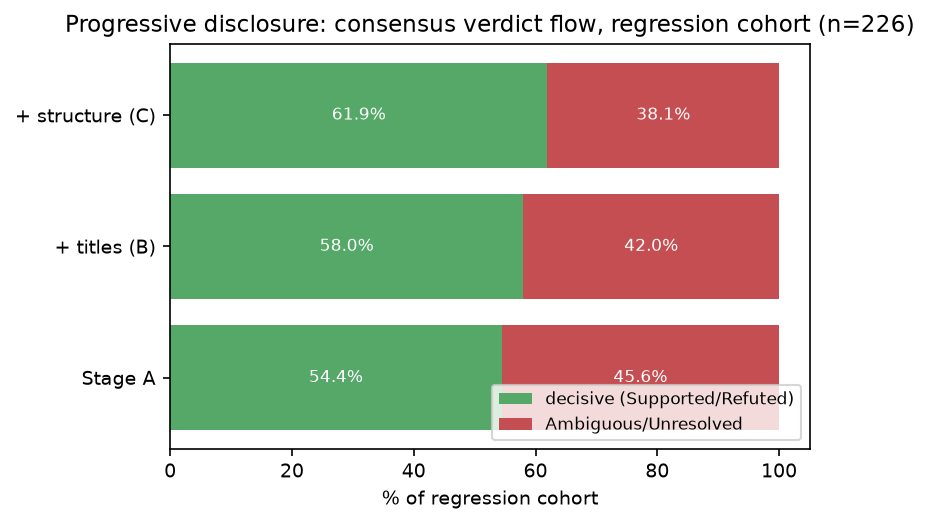
\includegraphics[width=0.85\linewidth]{../silver_adjudication_v1/cursor_panel/figures/fig3_resolution_flow.png}
\caption{Cursor/Grok resolution flow across Stages~A--C on the judged diagnostic cohort. Supplementary to Section~\ref{sec:rq3-grok}.}
\label{fig:flow}
\end{figure}

\begin{figure}[ht]
\centering
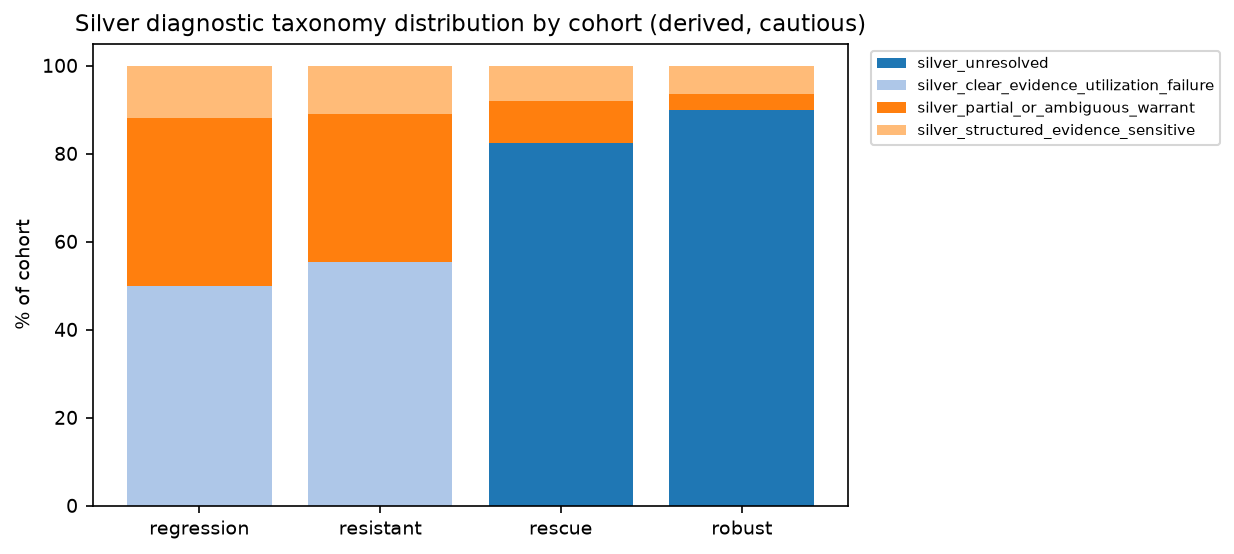
\includegraphics[width=0.75\linewidth]{../silver_adjudication_v1/cursor_panel/figures/fig7_taxonomy_distribution.png}
\caption{Cursor/Grok taxonomy distribution. Counts match Table~\ref{tab:mechanism-grok} on the 226 regressions.}
\label{fig:grok-tax}
\end{figure}

\begin{figure}[ht]
\centering
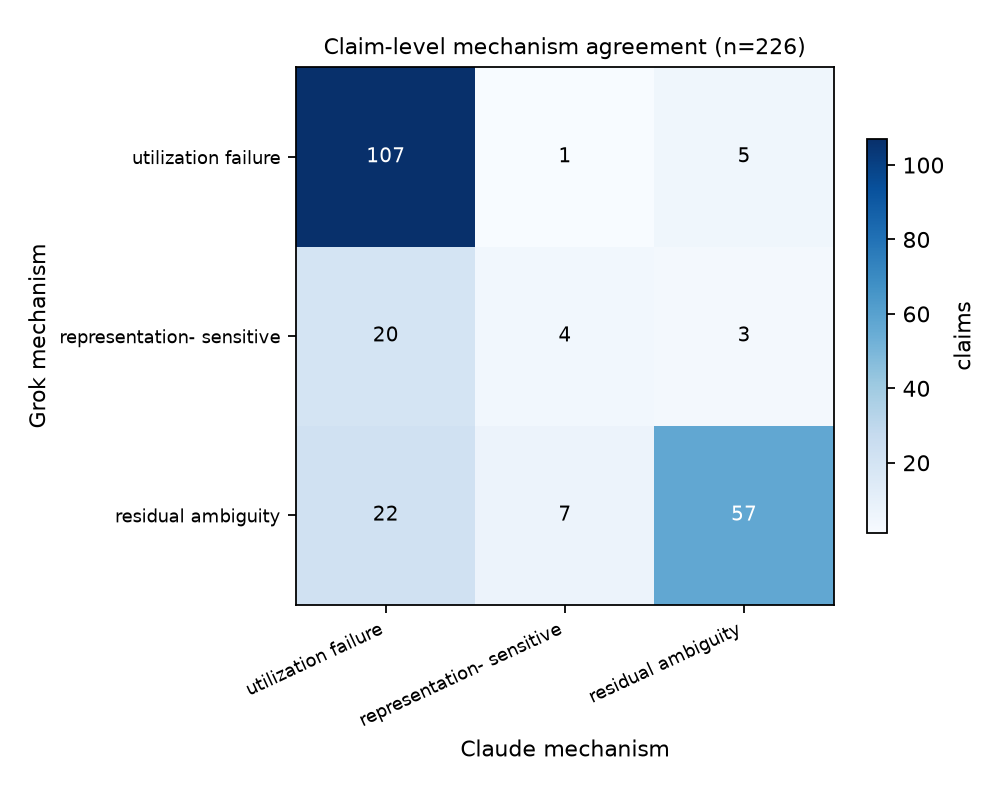
\includegraphics[width=0.88\linewidth]{../silver_adjudication_v1/claude_full_regression_panel/figures/fig3_mechanism_confusion.png}
\caption{Grok-versus-Claude taxonomy confusion on the 226 regressions. Disagreement is directional toward Claude utilization failure.}
\label{fig:confusion}
\end{figure}

\section{Denominator checklist}
\label{app:denoms}

\begin{tabular}{lr}
\toprule
Quantity & $n$ \\
\midrule
FEVER claims in the paired experiment & 10{,}000 \\
GPT predictions & 40{,}000 \\
Diagnostic-cohort claims constructed & 1{,}061 \\
Judged diagnostic-cohort items & 1{,}060 \\
Unique regressions & 226 \\
Grok Stage~C residual leftovers & 231 \\
Claude residual judgments & 1{,}155 \\
Claude full judgments & 3{,}390 \\
\bottomrule
\end{tabular}


\end{document}
